% Options for packages loaded elsewhere
\PassOptionsToPackage{unicode}{hyperref}
\PassOptionsToPackage{hyphens}{url}
\PassOptionsToPackage{dvipsnames,svgnames,x11names}{xcolor}
%
\documentclass[
  letterpaper,
  DIV=11,
  numbers=noendperiod]{scrartcl}

\usepackage{amsmath,amssymb}
\usepackage{lmodern}
\usepackage{iftex}
\ifPDFTeX
  \usepackage[T1]{fontenc}
  \usepackage[utf8]{inputenc}
  \usepackage{textcomp} % provide euro and other symbols
\else % if luatex or xetex
  \usepackage{unicode-math}
  \defaultfontfeatures{Scale=MatchLowercase}
  \defaultfontfeatures[\rmfamily]{Ligatures=TeX,Scale=1}
\fi
% Use upquote if available, for straight quotes in verbatim environments
\IfFileExists{upquote.sty}{\usepackage{upquote}}{}
\IfFileExists{microtype.sty}{% use microtype if available
  \usepackage[]{microtype}
  \UseMicrotypeSet[protrusion]{basicmath} % disable protrusion for tt fonts
}{}
\makeatletter
\@ifundefined{KOMAClassName}{% if non-KOMA class
  \IfFileExists{parskip.sty}{%
    \usepackage{parskip}
  }{% else
    \setlength{\parindent}{0pt}
    \setlength{\parskip}{6pt plus 2pt minus 1pt}}
}{% if KOMA class
  \KOMAoptions{parskip=half}}
\makeatother
\usepackage{xcolor}
\setlength{\emergencystretch}{3em} % prevent overfull lines
\setcounter{secnumdepth}{-\maxdimen} % remove section numbering
% Make \paragraph and \subparagraph free-standing
\ifx\paragraph\undefined\else
  \let\oldparagraph\paragraph
  \renewcommand{\paragraph}[1]{\oldparagraph{#1}\mbox{}}
\fi
\ifx\subparagraph\undefined\else
  \let\oldsubparagraph\subparagraph
  \renewcommand{\subparagraph}[1]{\oldsubparagraph{#1}\mbox{}}
\fi

\usepackage{color}
\usepackage{fancyvrb}
\newcommand{\VerbBar}{|}
\newcommand{\VERB}{\Verb[commandchars=\\\{\}]}
\DefineVerbatimEnvironment{Highlighting}{Verbatim}{commandchars=\\\{\}}
% Add ',fontsize=\small' for more characters per line
\usepackage{framed}
\definecolor{shadecolor}{RGB}{241,243,245}
\newenvironment{Shaded}{\begin{snugshade}}{\end{snugshade}}
\newcommand{\AlertTok}[1]{\textcolor[rgb]{0.68,0.00,0.00}{#1}}
\newcommand{\AnnotationTok}[1]{\textcolor[rgb]{0.37,0.37,0.37}{#1}}
\newcommand{\AttributeTok}[1]{\textcolor[rgb]{0.40,0.45,0.13}{#1}}
\newcommand{\BaseNTok}[1]{\textcolor[rgb]{0.68,0.00,0.00}{#1}}
\newcommand{\BuiltInTok}[1]{\textcolor[rgb]{0.00,0.23,0.31}{#1}}
\newcommand{\CharTok}[1]{\textcolor[rgb]{0.13,0.47,0.30}{#1}}
\newcommand{\CommentTok}[1]{\textcolor[rgb]{0.37,0.37,0.37}{#1}}
\newcommand{\CommentVarTok}[1]{\textcolor[rgb]{0.37,0.37,0.37}{\textit{#1}}}
\newcommand{\ConstantTok}[1]{\textcolor[rgb]{0.56,0.35,0.01}{#1}}
\newcommand{\ControlFlowTok}[1]{\textcolor[rgb]{0.00,0.23,0.31}{#1}}
\newcommand{\DataTypeTok}[1]{\textcolor[rgb]{0.68,0.00,0.00}{#1}}
\newcommand{\DecValTok}[1]{\textcolor[rgb]{0.68,0.00,0.00}{#1}}
\newcommand{\DocumentationTok}[1]{\textcolor[rgb]{0.37,0.37,0.37}{\textit{#1}}}
\newcommand{\ErrorTok}[1]{\textcolor[rgb]{0.68,0.00,0.00}{#1}}
\newcommand{\ExtensionTok}[1]{\textcolor[rgb]{0.00,0.23,0.31}{#1}}
\newcommand{\FloatTok}[1]{\textcolor[rgb]{0.68,0.00,0.00}{#1}}
\newcommand{\FunctionTok}[1]{\textcolor[rgb]{0.28,0.35,0.67}{#1}}
\newcommand{\ImportTok}[1]{\textcolor[rgb]{0.00,0.46,0.62}{#1}}
\newcommand{\InformationTok}[1]{\textcolor[rgb]{0.37,0.37,0.37}{#1}}
\newcommand{\KeywordTok}[1]{\textcolor[rgb]{0.00,0.23,0.31}{#1}}
\newcommand{\NormalTok}[1]{\textcolor[rgb]{0.00,0.23,0.31}{#1}}
\newcommand{\OperatorTok}[1]{\textcolor[rgb]{0.37,0.37,0.37}{#1}}
\newcommand{\OtherTok}[1]{\textcolor[rgb]{0.00,0.23,0.31}{#1}}
\newcommand{\PreprocessorTok}[1]{\textcolor[rgb]{0.68,0.00,0.00}{#1}}
\newcommand{\RegionMarkerTok}[1]{\textcolor[rgb]{0.00,0.23,0.31}{#1}}
\newcommand{\SpecialCharTok}[1]{\textcolor[rgb]{0.37,0.37,0.37}{#1}}
\newcommand{\SpecialStringTok}[1]{\textcolor[rgb]{0.13,0.47,0.30}{#1}}
\newcommand{\StringTok}[1]{\textcolor[rgb]{0.13,0.47,0.30}{#1}}
\newcommand{\VariableTok}[1]{\textcolor[rgb]{0.07,0.07,0.07}{#1}}
\newcommand{\VerbatimStringTok}[1]{\textcolor[rgb]{0.13,0.47,0.30}{#1}}
\newcommand{\WarningTok}[1]{\textcolor[rgb]{0.37,0.37,0.37}{\textit{#1}}}

\providecommand{\tightlist}{%
  \setlength{\itemsep}{0pt}\setlength{\parskip}{0pt}}\usepackage{longtable,booktabs,array}
\usepackage{calc} % for calculating minipage widths
% Correct order of tables after \paragraph or \subparagraph
\usepackage{etoolbox}
\makeatletter
\patchcmd\longtable{\par}{\if@noskipsec\mbox{}\fi\par}{}{}
\makeatother
% Allow footnotes in longtable head/foot
\IfFileExists{footnotehyper.sty}{\usepackage{footnotehyper}}{\usepackage{footnote}}
\makesavenoteenv{longtable}
\usepackage{graphicx}
\makeatletter
\def\maxwidth{\ifdim\Gin@nat@width>\linewidth\linewidth\else\Gin@nat@width\fi}
\def\maxheight{\ifdim\Gin@nat@height>\textheight\textheight\else\Gin@nat@height\fi}
\makeatother
% Scale images if necessary, so that they will not overflow the page
% margins by default, and it is still possible to overwrite the defaults
% using explicit options in \includegraphics[width, height, ...]{}
\setkeys{Gin}{width=\maxwidth,height=\maxheight,keepaspectratio}
% Set default figure placement to htbp
\makeatletter
\def\fps@figure{htbp}
\makeatother

\KOMAoption{captions}{tableheading}
\makeatletter
\makeatother
\makeatletter
\makeatother
\makeatletter
\@ifpackageloaded{caption}{}{\usepackage{caption}}
\AtBeginDocument{%
\ifdefined\contentsname
  \renewcommand*\contentsname{Table of contents}
\else
  \newcommand\contentsname{Table of contents}
\fi
\ifdefined\listfigurename
  \renewcommand*\listfigurename{List of Figures}
\else
  \newcommand\listfigurename{List of Figures}
\fi
\ifdefined\listtablename
  \renewcommand*\listtablename{List of Tables}
\else
  \newcommand\listtablename{List of Tables}
\fi
\ifdefined\figurename
  \renewcommand*\figurename{Figure}
\else
  \newcommand\figurename{Figure}
\fi
\ifdefined\tablename
  \renewcommand*\tablename{Table}
\else
  \newcommand\tablename{Table}
\fi
}
\@ifpackageloaded{float}{}{\usepackage{float}}
\floatstyle{ruled}
\@ifundefined{c@chapter}{\newfloat{codelisting}{h}{lop}}{\newfloat{codelisting}{h}{lop}[chapter]}
\floatname{codelisting}{Listing}
\newcommand*\listoflistings{\listof{codelisting}{List of Listings}}
\makeatother
\makeatletter
\@ifpackageloaded{caption}{}{\usepackage{caption}}
\@ifpackageloaded{subcaption}{}{\usepackage{subcaption}}
\makeatother
\makeatletter
\@ifpackageloaded{tcolorbox}{}{\usepackage[many]{tcolorbox}}
\makeatother
\makeatletter
\@ifundefined{shadecolor}{\definecolor{shadecolor}{rgb}{.97, .97, .97}}
\makeatother
\makeatletter
\makeatother
\ifLuaTeX
  \usepackage{selnolig}  % disable illegal ligatures
\fi
\IfFileExists{bookmark.sty}{\usepackage{bookmark}}{\usepackage{hyperref}}
\IfFileExists{xurl.sty}{\usepackage{xurl}}{} % add URL line breaks if available
\urlstyle{same} % disable monospaced font for URLs
\hypersetup{
  pdftitle={Class 19: Pertussis Mini Project},
  pdfauthor={Eric Jordahl},
  colorlinks=true,
  linkcolor={blue},
  filecolor={Maroon},
  citecolor={Blue},
  urlcolor={Blue},
  pdfcreator={LaTeX via pandoc}}

\title{Class 19: Pertussis Mini Project}
\author{Eric Jordahl}
\date{2022-11-30}

\begin{document}
\maketitle
\ifdefined\Shaded\renewenvironment{Shaded}{\begin{tcolorbox}[interior hidden, breakable, enhanced, borderline west={3pt}{0pt}{shadecolor}, frame hidden, sharp corners, boxrule=0pt]}{\end{tcolorbox}}\fi

\renewcommand*\contentsname{Table of contents}
{
\hypersetup{linkcolor=}
\setcounter{tocdepth}{3}
\tableofcontents
}
\hypertarget{investigating-pertussis-cases-by-year}{%
\section{1. Investigating Pertussis Cases By
Year}\label{investigating-pertussis-cases-by-year}}

\hypertarget{q1}{%
\subsection{Q1}\label{q1}}

\textbf{With the help of the R ``addin'' package datapasta assign the
CDC pertussis case number data to a data frame called cdc and use ggplot
to make a plot of cases numbers over time}

\begin{Shaded}
\begin{Highlighting}[]
\CommentTok{\#use datapasta to paste copied CDC data table and paste it as dataframe.}
\NormalTok{cdc }\OtherTok{\textless{}{-}} \FunctionTok{data.frame}\NormalTok{(}
                          \AttributeTok{Year =} \FunctionTok{c}\NormalTok{(1922L,}
\NormalTok{                                   1923L,1924L,1925L,1926L,1927L,1928L,}
\NormalTok{                                   1929L,1930L,1931L,1932L,1933L,1934L,1935L,}
\NormalTok{                                   1936L,1937L,1938L,1939L,1940L,1941L,}
\NormalTok{                                   1942L,1943L,1944L,1945L,1946L,1947L,1948L,}
\NormalTok{                                   1949L,1950L,1951L,1952L,1953L,1954L,}
\NormalTok{                                   1955L,1956L,1957L,1958L,1959L,1960L,}
\NormalTok{                                   1961L,1962L,1963L,1964L,1965L,1966L,1967L,}
\NormalTok{                                   1968L,1969L,1970L,1971L,1972L,1973L,}
\NormalTok{                                   1974L,1975L,1976L,1977L,1978L,1979L,1980L,}
\NormalTok{                                   1981L,1982L,1983L,1984L,1985L,1986L,}
\NormalTok{                                   1987L,1988L,1989L,1990L,1991L,1992L,1993L,}
\NormalTok{                                   1994L,1995L,1996L,1997L,1998L,1999L,}
\NormalTok{                                   2000L,2001L,2002L,2003L,2004L,2005L,}
\NormalTok{                                   2006L,2007L,2008L,2009L,2010L,2011L,2012L,}
\NormalTok{                                   2013L,2014L,2015L,2016L,2017L,2018L,}
\NormalTok{                                   2019L),}
\AttributeTok{Cases =} \FunctionTok{c}\NormalTok{(}\DecValTok{107473}\NormalTok{,}
                                   \DecValTok{164191}\NormalTok{,}\DecValTok{165418}\NormalTok{,}\DecValTok{152003}\NormalTok{,}\DecValTok{202210}\NormalTok{,}\DecValTok{181411}\NormalTok{,}
                                   \DecValTok{161799}\NormalTok{,}\DecValTok{197371}\NormalTok{,}\DecValTok{166914}\NormalTok{,}\DecValTok{172559}\NormalTok{,}\DecValTok{215343}\NormalTok{,}\DecValTok{179135}\NormalTok{,}
                                   \DecValTok{265269}\NormalTok{,}\DecValTok{180518}\NormalTok{,}\DecValTok{147237}\NormalTok{,}\DecValTok{214652}\NormalTok{,}\DecValTok{227319}\NormalTok{,}\DecValTok{103188}\NormalTok{,}
                                   \DecValTok{183866}\NormalTok{,}\DecValTok{222202}\NormalTok{,}\DecValTok{191383}\NormalTok{,}\DecValTok{191890}\NormalTok{,}\DecValTok{109873}\NormalTok{,}
                                   \DecValTok{133792}\NormalTok{,}\DecValTok{109860}\NormalTok{,}\DecValTok{156517}\NormalTok{,}\DecValTok{74715}\NormalTok{,}\DecValTok{69479}\NormalTok{,}\DecValTok{120718}\NormalTok{,}
                                   \DecValTok{68687}\NormalTok{,}\DecValTok{45030}\NormalTok{,}\DecValTok{37129}\NormalTok{,}\DecValTok{60886}\NormalTok{,}\DecValTok{62786}\NormalTok{,}\DecValTok{31732}\NormalTok{,}\DecValTok{28295}\NormalTok{,}
                                   \DecValTok{32148}\NormalTok{,}\DecValTok{40005}\NormalTok{,}\DecValTok{14809}\NormalTok{,}\DecValTok{11468}\NormalTok{,}\DecValTok{17749}\NormalTok{,}\DecValTok{17135}\NormalTok{,}
                                   \DecValTok{13005}\NormalTok{,}\DecValTok{6799}\NormalTok{,}\DecValTok{7717}\NormalTok{,}\DecValTok{9718}\NormalTok{,}\DecValTok{4810}\NormalTok{,}\DecValTok{3285}\NormalTok{,}\DecValTok{4249}\NormalTok{,}
                                   \DecValTok{3036}\NormalTok{,}\DecValTok{3287}\NormalTok{,}\DecValTok{1759}\NormalTok{,}\DecValTok{2402}\NormalTok{,}\DecValTok{1738}\NormalTok{,}\DecValTok{1010}\NormalTok{,}\DecValTok{2177}\NormalTok{,}\DecValTok{2063}\NormalTok{,}
                                   \DecValTok{1623}\NormalTok{,}\DecValTok{1730}\NormalTok{,}\DecValTok{1248}\NormalTok{,}\DecValTok{1895}\NormalTok{,}\DecValTok{2463}\NormalTok{,}\DecValTok{2276}\NormalTok{,}\DecValTok{3589}\NormalTok{,}
                                   \DecValTok{4195}\NormalTok{,}\DecValTok{2823}\NormalTok{,}\DecValTok{3450}\NormalTok{,}\DecValTok{4157}\NormalTok{,}\DecValTok{4570}\NormalTok{,}\DecValTok{2719}\NormalTok{,}\DecValTok{4083}\NormalTok{,}\DecValTok{6586}\NormalTok{,}
                                   \DecValTok{4617}\NormalTok{,}\DecValTok{5137}\NormalTok{,}\DecValTok{7796}\NormalTok{,}\DecValTok{6564}\NormalTok{,}\DecValTok{7405}\NormalTok{,}\DecValTok{7298}\NormalTok{,}\DecValTok{7867}\NormalTok{,}
                                   \DecValTok{7580}\NormalTok{,}\DecValTok{9771}\NormalTok{,}\DecValTok{11647}\NormalTok{,}\DecValTok{25827}\NormalTok{,}\DecValTok{25616}\NormalTok{,}\DecValTok{15632}\NormalTok{,}\DecValTok{10454}\NormalTok{,}
                                   \DecValTok{13278}\NormalTok{,}\DecValTok{16858}\NormalTok{,}\DecValTok{27550}\NormalTok{,}\DecValTok{18719}\NormalTok{,}\DecValTok{48277}\NormalTok{,}\DecValTok{28639}\NormalTok{,}
                                   \DecValTok{32971}\NormalTok{,}\DecValTok{20762}\NormalTok{,}\DecValTok{17972}\NormalTok{,}\DecValTok{18975}\NormalTok{,}\DecValTok{15609}\NormalTok{,}\DecValTok{18617}\NormalTok{)}
\NormalTok{)}
\FunctionTok{head}\NormalTok{(cdc)}
\end{Highlighting}
\end{Shaded}

\begin{verbatim}
  Year  Cases
1 1922 107473
2 1923 164191
3 1924 165418
4 1925 152003
5 1926 202210
6 1927 181411
\end{verbatim}

\begin{Shaded}
\begin{Highlighting}[]
\FunctionTok{library}\NormalTok{(ggplot2)}
\FunctionTok{ggplot}\NormalTok{(}\AttributeTok{data =}\NormalTok{ cdc) }\SpecialCharTok{+} \FunctionTok{aes}\NormalTok{(}\AttributeTok{x=}\NormalTok{Year, }\AttributeTok{y=}\NormalTok{Cases) }\SpecialCharTok{+}
  \FunctionTok{geom\_point}\NormalTok{() }\SpecialCharTok{+}
  \FunctionTok{geom\_line}\NormalTok{() }\SpecialCharTok{+}
  \FunctionTok{labs}\NormalTok{(}\AttributeTok{title =} \StringTok{"Pertussis cases per year in the USA"}\NormalTok{)}
\end{Highlighting}
\end{Shaded}

\begin{figure}[H]

{\centering 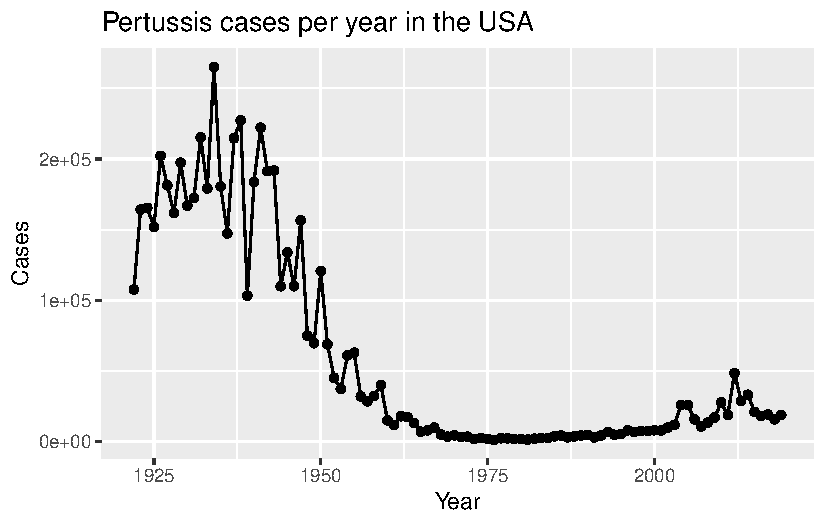
\includegraphics{Class19_files/figure-pdf/unnamed-chunk-2-1.pdf}

}

\end{figure}

\begin{Shaded}
\begin{Highlighting}[]
\NormalTok{baseplot }\OtherTok{\textless{}{-}} \FunctionTok{ggplot}\NormalTok{(}\AttributeTok{data =}\NormalTok{ cdc) }\SpecialCharTok{+} \FunctionTok{aes}\NormalTok{(}\AttributeTok{x=}\NormalTok{Year, }\AttributeTok{y=}\NormalTok{Cases) }\SpecialCharTok{+}
  \FunctionTok{geom\_point}\NormalTok{() }\SpecialCharTok{+}
  \FunctionTok{geom\_line}\NormalTok{() }\SpecialCharTok{+}
  \FunctionTok{labs}\NormalTok{(}\AttributeTok{title =} \StringTok{"Pertussis cases per year in the USA"}\NormalTok{)}
\end{Highlighting}
\end{Shaded}

\hypertarget{a-tale-of-two-vaccines}{%
\section{2. A Tale of Two Vaccines}\label{a-tale-of-two-vaccines}}

\#\#Q2 \textbf{Using the ggplot geom\_vline() function add lines to your
previous plot for the 1946 introduction of the wP vaccine and the 1996
switch to aP vaccine (see example in the hint below). What do you
notice?}

\begin{Shaded}
\begin{Highlighting}[]
\FunctionTok{library}\NormalTok{(ggplot2)}
\FunctionTok{ggplot}\NormalTok{(}\AttributeTok{data =}\NormalTok{ cdc) }\SpecialCharTok{+} \FunctionTok{aes}\NormalTok{(}\AttributeTok{x=}\NormalTok{Year, }\AttributeTok{y=}\NormalTok{Cases) }\SpecialCharTok{+}
  \FunctionTok{geom\_point}\NormalTok{() }\SpecialCharTok{+}
  \FunctionTok{geom\_line}\NormalTok{() }\SpecialCharTok{+}
  \FunctionTok{geom\_vline}\NormalTok{(}\AttributeTok{xintercept =} \DecValTok{1946}\NormalTok{, }\AttributeTok{color=}\StringTok{"RED"}\NormalTok{, }\AttributeTok{linetype =} \StringTok{"dotted"}\NormalTok{) }\SpecialCharTok{+}
  \FunctionTok{geom\_vline}\NormalTok{(}\AttributeTok{xintercept =} \DecValTok{1996}\NormalTok{, }\AttributeTok{color=}\StringTok{"BLUE"}\NormalTok{, }\AttributeTok{linetype =} \StringTok{"dotted"}\NormalTok{) }\SpecialCharTok{+}
  \FunctionTok{labs}\NormalTok{(}\AttributeTok{title =} \StringTok{"Pertussis cases per year in the USA"}\NormalTok{)}
\end{Highlighting}
\end{Shaded}

\begin{figure}[H]

{\centering 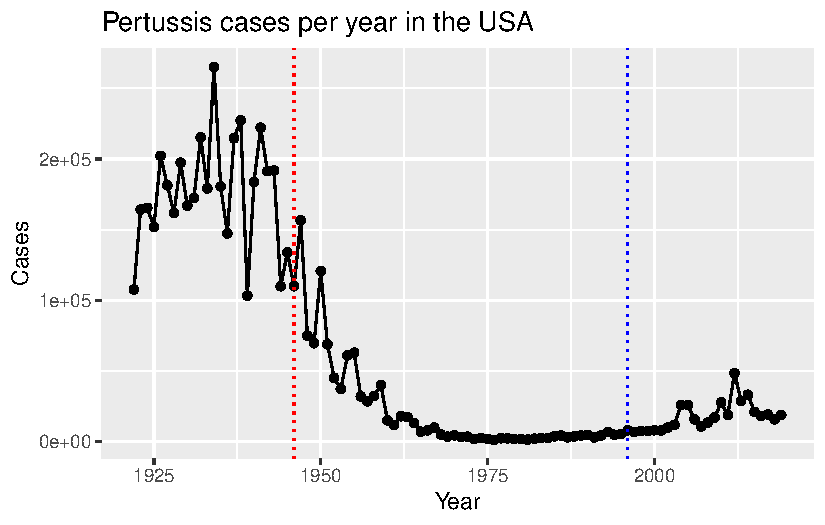
\includegraphics{Class19_files/figure-pdf/unnamed-chunk-3-1.pdf}

}

\end{figure}

\begin{Shaded}
\begin{Highlighting}[]
\NormalTok{baseplot }\OtherTok{\textless{}{-}} \FunctionTok{ggplot}\NormalTok{(}\AttributeTok{data =}\NormalTok{ cdc) }\SpecialCharTok{+} \FunctionTok{aes}\NormalTok{(}\AttributeTok{x=}\NormalTok{Year, }\AttributeTok{y=}\NormalTok{Cases) }\SpecialCharTok{+}
  \FunctionTok{geom\_point}\NormalTok{() }\SpecialCharTok{+}
  \FunctionTok{geom\_line}\NormalTok{() }\SpecialCharTok{+}
  \FunctionTok{labs}\NormalTok{(}\AttributeTok{title =} \StringTok{"Pertussis cases per year in the USA"}\NormalTok{)}
\end{Highlighting}
\end{Shaded}

\hypertarget{q3}{%
\subsection{Q3}\label{q3}}

\textbf{Describe what happened after the introduction of the aP vaccine?
Do you have a possible explanation for the observed trend?}

After the introduction of the aP vaccine, cases seemed to increase
slowly, but not to as large of numbers as before the wP vaccine. A
possible explanation for this trend is the resistance to administering
vaccines that has occurred more recently, or the new aP vaccine is less
efficient at preventing pertussis than the wP vaccine.

\hypertarget{exploring-cmi-pb-data}{%
\section{3. Exploring CMI-PB data}\label{exploring-cmi-pb-data}}

\begin{Shaded}
\begin{Highlighting}[]
\FunctionTok{library}\NormalTok{(jsonlite)}
\NormalTok{subject }\OtherTok{\textless{}{-}} \FunctionTok{read\_json}\NormalTok{(}\StringTok{"https://www.cmi{-}pb.org/api/subject"}\NormalTok{, }\AttributeTok{simplifyVector =} \ConstantTok{TRUE}\NormalTok{) }
\FunctionTok{head}\NormalTok{(subject, }\DecValTok{3}\NormalTok{)}
\end{Highlighting}
\end{Shaded}

\begin{verbatim}
  subject_id infancy_vac biological_sex              ethnicity  race
1          1          wP         Female Not Hispanic or Latino White
2          2          wP         Female Not Hispanic or Latino White
3          3          wP         Female                Unknown White
  year_of_birth date_of_boost      dataset
1    1986-01-01    2016-09-12 2020_dataset
2    1968-01-01    2019-01-28 2020_dataset
3    1983-01-01    2016-10-10 2020_dataset
\end{verbatim}

\hypertarget{q4}{%
\subsection{Q4}\label{q4}}

\textbf{How many aP and wP infancy vaccinated subjects are in the
dataset?}

\begin{Shaded}
\begin{Highlighting}[]
\FunctionTok{table}\NormalTok{(subject}\SpecialCharTok{$}\NormalTok{infancy\_vac)}
\end{Highlighting}
\end{Shaded}

\begin{verbatim}

aP wP 
47 49 
\end{verbatim}

There are 47 subjects in the aP dataset and 49 in the wP dataset

\hypertarget{q5}{%
\subsection{Q5}\label{q5}}

**How many Male and Female subjects/patients are in the dataset?

\begin{Shaded}
\begin{Highlighting}[]
\FunctionTok{table}\NormalTok{(subject}\SpecialCharTok{$}\NormalTok{biological\_sex)}
\end{Highlighting}
\end{Shaded}

\begin{verbatim}

Female   Male 
    66     30 
\end{verbatim}

There are 66 female subjescts and 30 male subjects

\hypertarget{q6}{%
\subsection{Q6}\label{q6}}

\textbf{What is the breakdown of race and biological sex (e.g.~number of
Asian females, White males etc\ldots)?}

\begin{Shaded}
\begin{Highlighting}[]
\FunctionTok{table}\NormalTok{(subject}\SpecialCharTok{$}\NormalTok{race, subject}\SpecialCharTok{$}\NormalTok{biological\_sex)}
\end{Highlighting}
\end{Shaded}

\begin{verbatim}
                                           
                                            Female Male
  American Indian/Alaska Native                  0    1
  Asian                                         18    9
  Black or African American                      2    0
  More Than One Race                             8    2
  Native Hawaiian or Other Pacific Islander      1    1
  Unknown or Not Reported                       10    4
  White                                         27   13
\end{verbatim}

\hypertarget{working-with-dates}{%
\subsection{Working with Dates}\label{working-with-dates}}

\begin{Shaded}
\begin{Highlighting}[]
\FunctionTok{library}\NormalTok{(lubridate)}
\end{Highlighting}
\end{Shaded}

\begin{verbatim}
Loading required package: timechange
\end{verbatim}

\begin{verbatim}

Attaching package: 'lubridate'
\end{verbatim}

\begin{verbatim}
The following objects are masked from 'package:base':

    date, intersect, setdiff, union
\end{verbatim}

\begin{Shaded}
\begin{Highlighting}[]
\FunctionTok{today}\NormalTok{()}
\end{Highlighting}
\end{Shaded}

\begin{verbatim}
[1] "2022-12-04"
\end{verbatim}

\begin{Shaded}
\begin{Highlighting}[]
\FunctionTok{library}\NormalTok{(lubridate)}
\FunctionTok{today}\NormalTok{() }\SpecialCharTok{{-}} \FunctionTok{ymd}\NormalTok{(}\StringTok{"2000{-}01{-}01"}\NormalTok{)}
\end{Highlighting}
\end{Shaded}

\begin{verbatim}
Time difference of 8373 days
\end{verbatim}

\begin{Shaded}
\begin{Highlighting}[]
\FunctionTok{library}\NormalTok{(lubridate)}
\FunctionTok{time\_length}\NormalTok{( }\FunctionTok{today}\NormalTok{() }\SpecialCharTok{{-}} \FunctionTok{ymd}\NormalTok{(}\StringTok{"2000{-}01{-}01"}\NormalTok{),  }\StringTok{"years"}\NormalTok{)}
\end{Highlighting}
\end{Shaded}

\begin{verbatim}
[1] 22.92402
\end{verbatim}

\hypertarget{q7}{%
\subsection{Q7}\label{q7}}

\textbf{Using this approach determine (i) the average age of wP
individuals, (ii) the average age of aP individuals; and (iii) are they
significantly different?}

\begin{Shaded}
\begin{Highlighting}[]
\NormalTok{subject}\SpecialCharTok{$}\NormalTok{age }\OtherTok{\textless{}{-}} \FunctionTok{today}\NormalTok{() }\SpecialCharTok{{-}} \FunctionTok{ymd}\NormalTok{(subject}\SpecialCharTok{$}\NormalTok{year\_of\_birth)}
\end{Highlighting}
\end{Shaded}

\begin{Shaded}
\begin{Highlighting}[]
\FunctionTok{library}\NormalTok{(dplyr)}
\end{Highlighting}
\end{Shaded}

\begin{verbatim}

Attaching package: 'dplyr'
\end{verbatim}

\begin{verbatim}
The following objects are masked from 'package:stats':

    filter, lag
\end{verbatim}

\begin{verbatim}
The following objects are masked from 'package:base':

    intersect, setdiff, setequal, union
\end{verbatim}

\begin{Shaded}
\begin{Highlighting}[]
\NormalTok{ap }\OtherTok{\textless{}{-}}\NormalTok{ subject }\SpecialCharTok{\%\textgreater{}\%} \FunctionTok{filter}\NormalTok{(infancy\_vac }\SpecialCharTok{==} \StringTok{"aP"}\NormalTok{)}

\FunctionTok{round}\NormalTok{( }\FunctionTok{summary}\NormalTok{( }\FunctionTok{time\_length}\NormalTok{( ap}\SpecialCharTok{$}\NormalTok{age, }\StringTok{"years"}\NormalTok{ ) ) )}
\end{Highlighting}
\end{Shaded}

\begin{verbatim}
   Min. 1st Qu.  Median    Mean 3rd Qu.    Max. 
     23      25      26      25      26      27 
\end{verbatim}

\begin{Shaded}
\begin{Highlighting}[]
\NormalTok{wp }\OtherTok{\textless{}{-}}\NormalTok{ subject }\SpecialCharTok{\%\textgreater{}\%} \FunctionTok{filter}\NormalTok{(infancy\_vac }\SpecialCharTok{==} \StringTok{"wP"}\NormalTok{)}
\FunctionTok{round}\NormalTok{( }\FunctionTok{summary}\NormalTok{( }\FunctionTok{time\_length}\NormalTok{( wp}\SpecialCharTok{$}\NormalTok{age, }\StringTok{"years"}\NormalTok{ ) ) )}
\end{Highlighting}
\end{Shaded}

\begin{verbatim}
   Min. 1st Qu.  Median    Mean 3rd Qu.    Max. 
     28      32      35      36      40      55 
\end{verbatim}

\hypertarget{q8}{%
\subsection{Q8}\label{q8}}

\textbf{Determine the age of all individuals at time of boost?}

\begin{Shaded}
\begin{Highlighting}[]
\NormalTok{int }\OtherTok{\textless{}{-}} \FunctionTok{ymd}\NormalTok{(subject}\SpecialCharTok{$}\NormalTok{date\_of\_boost) }\SpecialCharTok{{-}} \FunctionTok{ymd}\NormalTok{(subject}\SpecialCharTok{$}\NormalTok{year\_of\_birth)}
\NormalTok{age\_at\_boost }\OtherTok{\textless{}{-}} \FunctionTok{time\_length}\NormalTok{(int, }\StringTok{"year"}\NormalTok{)}
\FunctionTok{head}\NormalTok{(age\_at\_boost)}
\end{Highlighting}
\end{Shaded}

\begin{verbatim}
[1] 30.69678 51.07461 33.77413 28.65982 25.65914 28.77481
\end{verbatim}

\hypertarget{q9}{%
\subsection{Q9}\label{q9}}

\textbf{With the help of a faceted boxplot or histogram (see below), do
you think these two groups are significantly different?}

\begin{Shaded}
\begin{Highlighting}[]
\FunctionTok{ggplot}\NormalTok{(subject) }\SpecialCharTok{+}
  \FunctionTok{aes}\NormalTok{(}\FunctionTok{time\_length}\NormalTok{(age, }\StringTok{"year"}\NormalTok{),}
      \AttributeTok{fill=}\FunctionTok{as.factor}\NormalTok{(infancy\_vac)) }\SpecialCharTok{+}
  \FunctionTok{geom\_histogram}\NormalTok{(}\AttributeTok{show.legend=}\ConstantTok{FALSE}\NormalTok{) }\SpecialCharTok{+}
  \FunctionTok{facet\_wrap}\NormalTok{(}\FunctionTok{vars}\NormalTok{(infancy\_vac), }\AttributeTok{nrow=}\DecValTok{2}\NormalTok{) }
\end{Highlighting}
\end{Shaded}

\begin{verbatim}
`stat_bin()` using `bins = 30`. Pick better value with `binwidth`.
\end{verbatim}

\begin{figure}[H]

{\centering 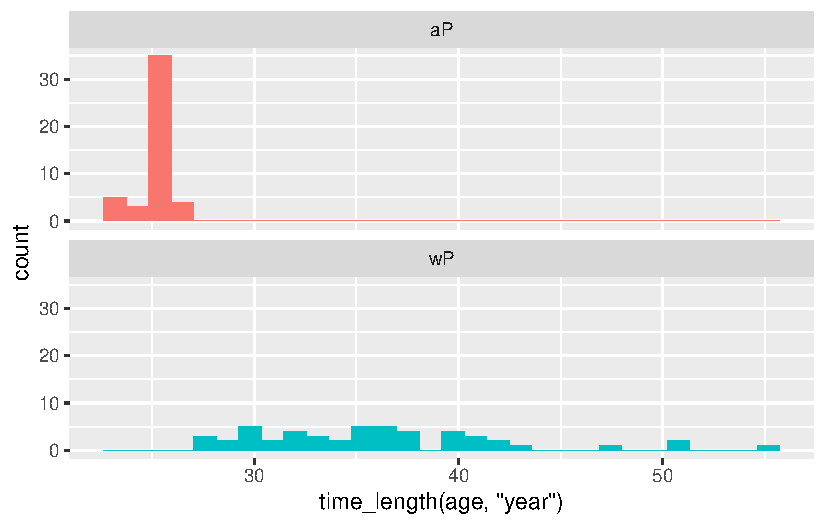
\includegraphics{Class19_files/figure-pdf/unnamed-chunk-15-1.pdf}

}

\end{figure}

\hypertarget{joining-multiple-tables}{%
\subsection{Joining multiple tables}\label{joining-multiple-tables}}

\begin{Shaded}
\begin{Highlighting}[]
\CommentTok{\# Complete the API URLs...}
\NormalTok{specimen }\OtherTok{\textless{}{-}} \FunctionTok{read\_json}\NormalTok{(}\StringTok{"http://cmi{-}pb.org/api/specimen"}\NormalTok{, }\AttributeTok{simplifyVector =} \ConstantTok{TRUE}\NormalTok{)}
\FunctionTok{head}\NormalTok{(specimen)}
\end{Highlighting}
\end{Shaded}

\begin{verbatim}
  specimen_id subject_id actual_day_relative_to_boost
1           1          1                           -3
2           2          1                          736
3           3          1                            1
4           4          1                            3
5           5          1                            7
6           6          1                           11
  planned_day_relative_to_boost specimen_type visit
1                             0         Blood     1
2                           736         Blood    10
3                             1         Blood     2
4                             3         Blood     3
5                             7         Blood     4
6                            14         Blood     5
\end{verbatim}

\hypertarget{q9-1}{%
\subsection{Q9}\label{q9-1}}

\textbf{Complete the code to join specimen and subject tables to make a
new merged data frame containing all specimen records along with their
associated subject details}

\begin{Shaded}
\begin{Highlighting}[]
\NormalTok{meta }\OtherTok{\textless{}{-}} \FunctionTok{inner\_join}\NormalTok{(specimen, subject)}
\end{Highlighting}
\end{Shaded}

\begin{verbatim}
Joining, by = "subject_id"
\end{verbatim}

\begin{Shaded}
\begin{Highlighting}[]
\FunctionTok{dim}\NormalTok{(meta)}
\end{Highlighting}
\end{Shaded}

\begin{verbatim}
[1] 729  14
\end{verbatim}

\hypertarget{q10}{%
\subsection{Q10}\label{q10}}

\textbf{Now using the same procedure join meta with titer data so we can
further analyze this data in terms of time of visit aP/wP, male/female
etc.}

\begin{Shaded}
\begin{Highlighting}[]
\NormalTok{titer }\OtherTok{\textless{}{-}} \FunctionTok{read\_json}\NormalTok{(}\StringTok{"http://cmi{-}pb.org/api/ab\_titer"}\NormalTok{, }\AttributeTok{simplifyVector =} \ConstantTok{TRUE}\NormalTok{)}
\FunctionTok{head}\NormalTok{(titer)}
\end{Highlighting}
\end{Shaded}

\begin{verbatim}
  specimen_id isotype is_antigen_specific antigen        MFI MFI_normalised
1           1     IgE               FALSE   Total 1110.21154       2.493425
2           1     IgE               FALSE   Total 2708.91616       2.493425
3           1     IgG                TRUE      PT   68.56614       3.736992
4           1     IgG                TRUE     PRN  332.12718       2.602350
5           1     IgG                TRUE     FHA 1887.12263      34.050956
6           1     IgE                TRUE     ACT    0.10000       1.000000
   unit lower_limit_of_detection
1 UG/ML                 2.096133
2 IU/ML                29.170000
3 IU/ML                 0.530000
4 IU/ML                 6.205949
5 IU/ML                 4.679535
6 IU/ML                 2.816431
\end{verbatim}

\begin{Shaded}
\begin{Highlighting}[]
\NormalTok{abdata }\OtherTok{\textless{}{-}} \FunctionTok{inner\_join}\NormalTok{(titer, meta)}
\end{Highlighting}
\end{Shaded}

\begin{verbatim}
Joining, by = "specimen_id"
\end{verbatim}

\begin{Shaded}
\begin{Highlighting}[]
\FunctionTok{dim}\NormalTok{(abdata)}
\end{Highlighting}
\end{Shaded}

\begin{verbatim}
[1] 32675    21
\end{verbatim}

\hypertarget{q11}{%
\subsection{Q11}\label{q11}}

\textbf{How many specimens (i.e.~entries in abdata) do we have for each
isotype?}

\begin{Shaded}
\begin{Highlighting}[]
\FunctionTok{table}\NormalTok{(abdata}\SpecialCharTok{$}\NormalTok{isotype)}
\end{Highlighting}
\end{Shaded}

\begin{verbatim}

 IgE  IgG IgG1 IgG2 IgG3 IgG4 
6698 1413 6141 6141 6141 6141 
\end{verbatim}

\hypertarget{q12}{%
\subsection{Q12}\label{q12}}

\textbf{What do you notice about the number of visit 8 specimens
compared to other visits?}

\begin{Shaded}
\begin{Highlighting}[]
\FunctionTok{table}\NormalTok{(abdata}\SpecialCharTok{$}\NormalTok{visit)}
\end{Highlighting}
\end{Shaded}

\begin{verbatim}

   1    2    3    4    5    6    7    8 
5795 4640 4640 4640 4640 4320 3920   80 
\end{verbatim}

The eighth visit had way less specimens in comparison to the other 7
visits.

\hypertarget{examine-igg1-ab-titer-levels}{%
\section{4. Examine IgG1 Ab titer
levels}\label{examine-igg1-ab-titer-levels}}

\hypertarget{q13}{%
\subsection{Q13}\label{q13}}

\textbf{Complete the following code to make a summary boxplot of Ab
titer levels (MFI) for all antigens}

\begin{Shaded}
\begin{Highlighting}[]
\NormalTok{ig1 }\OtherTok{\textless{}{-}}\NormalTok{ abdata }\SpecialCharTok{\%\textgreater{}\%} \FunctionTok{filter}\NormalTok{(isotype }\SpecialCharTok{==} \StringTok{"IgG1"}\NormalTok{, visit}\SpecialCharTok{!=}\DecValTok{8}\NormalTok{)}
\FunctionTok{head}\NormalTok{(ig1)}
\end{Highlighting}
\end{Shaded}

\begin{verbatim}
  specimen_id isotype is_antigen_specific antigen        MFI MFI_normalised
1           1    IgG1                TRUE     ACT 274.355068      0.6928058
2           1    IgG1                TRUE     LOS  10.974026      2.1645083
3           1    IgG1                TRUE   FELD1   1.448796      0.8080941
4           1    IgG1                TRUE   BETV1   0.100000      1.0000000
5           1    IgG1                TRUE   LOLP1   0.100000      1.0000000
6           1    IgG1                TRUE Measles  36.277417      1.6638332
   unit lower_limit_of_detection subject_id actual_day_relative_to_boost
1 IU/ML                 3.848750          1                           -3
2 IU/ML                 4.357917          1                           -3
3 IU/ML                 2.699944          1                           -3
4 IU/ML                 1.734784          1                           -3
5 IU/ML                 2.550606          1                           -3
6 IU/ML                 4.438966          1                           -3
  planned_day_relative_to_boost specimen_type visit infancy_vac biological_sex
1                             0         Blood     1          wP         Female
2                             0         Blood     1          wP         Female
3                             0         Blood     1          wP         Female
4                             0         Blood     1          wP         Female
5                             0         Blood     1          wP         Female
6                             0         Blood     1          wP         Female
               ethnicity  race year_of_birth date_of_boost      dataset
1 Not Hispanic or Latino White    1986-01-01    2016-09-12 2020_dataset
2 Not Hispanic or Latino White    1986-01-01    2016-09-12 2020_dataset
3 Not Hispanic or Latino White    1986-01-01    2016-09-12 2020_dataset
4 Not Hispanic or Latino White    1986-01-01    2016-09-12 2020_dataset
5 Not Hispanic or Latino White    1986-01-01    2016-09-12 2020_dataset
6 Not Hispanic or Latino White    1986-01-01    2016-09-12 2020_dataset
         age
1 13486 days
2 13486 days
3 13486 days
4 13486 days
5 13486 days
6 13486 days
\end{verbatim}

\begin{Shaded}
\begin{Highlighting}[]
\FunctionTok{ggplot}\NormalTok{(ig1) }\SpecialCharTok{+}
  \FunctionTok{aes}\NormalTok{(MFI, antigen, }\AttributeTok{color=}\NormalTok{ antigen) }\SpecialCharTok{+}
  \FunctionTok{geom\_boxplot}\NormalTok{() }\SpecialCharTok{+}
  \FunctionTok{facet\_wrap}\NormalTok{(}\FunctionTok{vars}\NormalTok{(visit), }\AttributeTok{nrow=}\DecValTok{2}\NormalTok{) }\SpecialCharTok{+}
  \FunctionTok{theme}\NormalTok{(}\AttributeTok{axis.text.x =} \FunctionTok{element\_text}\NormalTok{(}\AttributeTok{angle =} \DecValTok{45}\NormalTok{, }\AttributeTok{hjust=}\DecValTok{1}\NormalTok{))}
\end{Highlighting}
\end{Shaded}

\begin{figure}[H]

{\centering 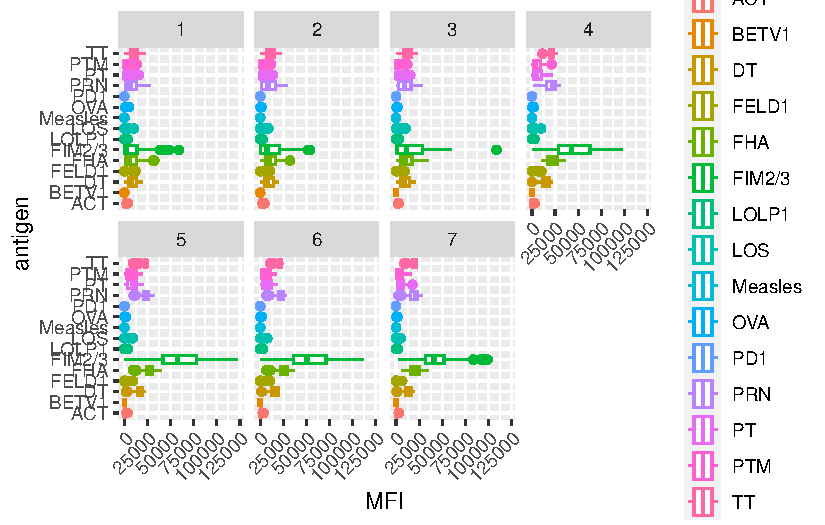
\includegraphics{Class19_files/figure-pdf/unnamed-chunk-23-1.pdf}

}

\end{figure}

\hypertarget{q14}{%
\subsection{Q14}\label{q14}}

\textbf{What antigens show differences in the level of IgG1 antibody
titers recognizing them over time? Why these and not others?}

FIM2/3 appears to have the most different titer level for these
antigens. This could be because it could be the only immunodominant
antigen, or it could be more accessible than other antigens.

\begin{Shaded}
\begin{Highlighting}[]
\FunctionTok{ggplot}\NormalTok{(ig1) }\SpecialCharTok{+}
  \FunctionTok{aes}\NormalTok{(MFI, antigen, }\AttributeTok{col=}\NormalTok{infancy\_vac ) }\SpecialCharTok{+}
  \FunctionTok{geom\_boxplot}\NormalTok{(}\AttributeTok{show.legend =} \ConstantTok{FALSE}\NormalTok{) }\SpecialCharTok{+} 
  \FunctionTok{facet\_wrap}\NormalTok{(}\FunctionTok{vars}\NormalTok{(visit), }\AttributeTok{nrow=}\DecValTok{2}\NormalTok{) }\SpecialCharTok{+}
  \FunctionTok{theme\_bw}\NormalTok{()}
\end{Highlighting}
\end{Shaded}

\begin{figure}[H]

{\centering 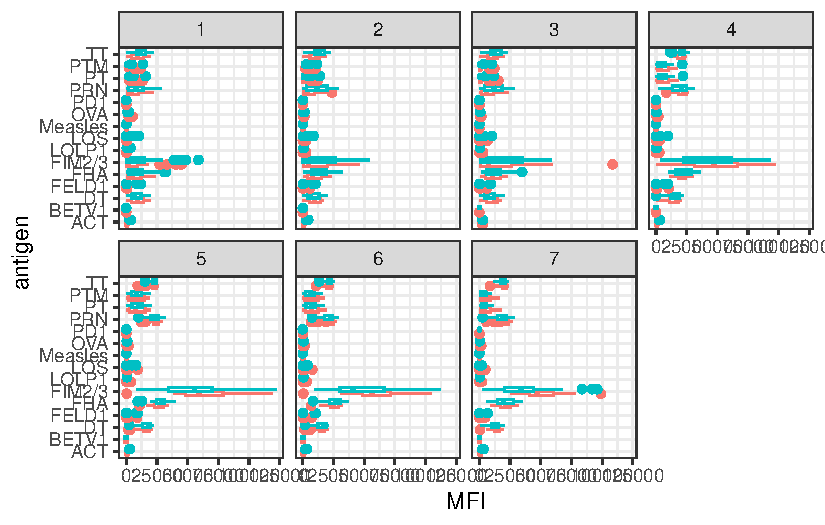
\includegraphics{Class19_files/figure-pdf/unnamed-chunk-24-1.pdf}

}

\end{figure}

\begin{Shaded}
\begin{Highlighting}[]
\FunctionTok{ggplot}\NormalTok{(ig1) }\SpecialCharTok{+}
  \FunctionTok{aes}\NormalTok{(MFI, antigen, }\AttributeTok{col=}\NormalTok{infancy\_vac ) }\SpecialCharTok{+}
  \FunctionTok{geom\_boxplot}\NormalTok{(}\AttributeTok{show.legend =} \ConstantTok{FALSE}\NormalTok{) }\SpecialCharTok{+} 
  \FunctionTok{facet\_wrap}\NormalTok{(}\FunctionTok{vars}\NormalTok{(infancy\_vac, visit), }\AttributeTok{nrow=}\DecValTok{2}\NormalTok{)}
\end{Highlighting}
\end{Shaded}

\begin{figure}[H]

{\centering 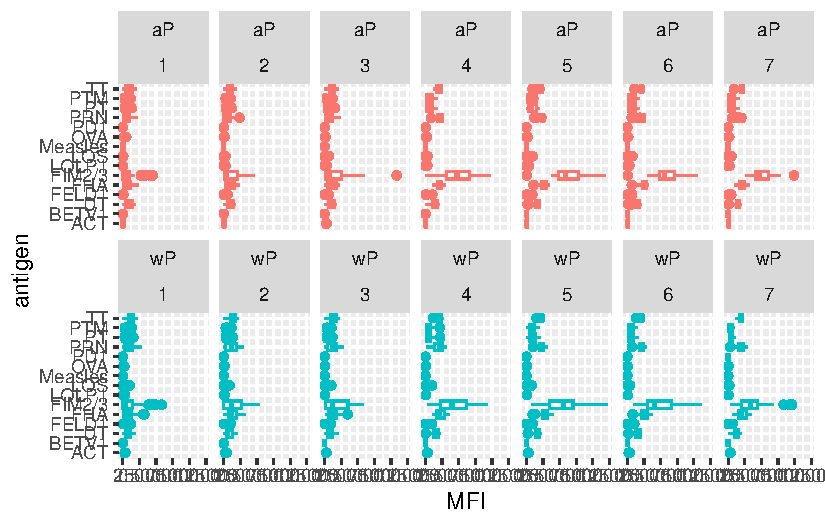
\includegraphics{Class19_files/figure-pdf/unnamed-chunk-25-1.pdf}

}

\end{figure}

\hypertarget{q15}{%
\subsection{Q15}\label{q15}}

\textbf{Filter to pull out only two specific antigens for analysis and
create a boxplot for each. You can chose any you like. Below I picked a
``control'' antigen (``Measles'', that is not in our vaccines) and a
clear antigen of interest (``FIM2/3'', extra-cellular fimbriae proteins
from B. pertussis that participate in substrate attachment).}

\begin{Shaded}
\begin{Highlighting}[]
\FunctionTok{filter}\NormalTok{(ig1, antigen}\SpecialCharTok{==}\StringTok{"Measles"}\NormalTok{) }\SpecialCharTok{\%\textgreater{}\%}
  \FunctionTok{ggplot}\NormalTok{() }\SpecialCharTok{+}
  \FunctionTok{aes}\NormalTok{(MFI, }\AttributeTok{col=}\NormalTok{infancy\_vac) }\SpecialCharTok{+}
  \FunctionTok{geom\_boxplot}\NormalTok{(}\AttributeTok{show.legend =}\NormalTok{ F) }\SpecialCharTok{+}
  \FunctionTok{facet\_wrap}\NormalTok{(}\FunctionTok{vars}\NormalTok{(visit)) }\SpecialCharTok{+}
  \FunctionTok{theme\_bw}\NormalTok{()}
\end{Highlighting}
\end{Shaded}

\begin{figure}[H]

{\centering 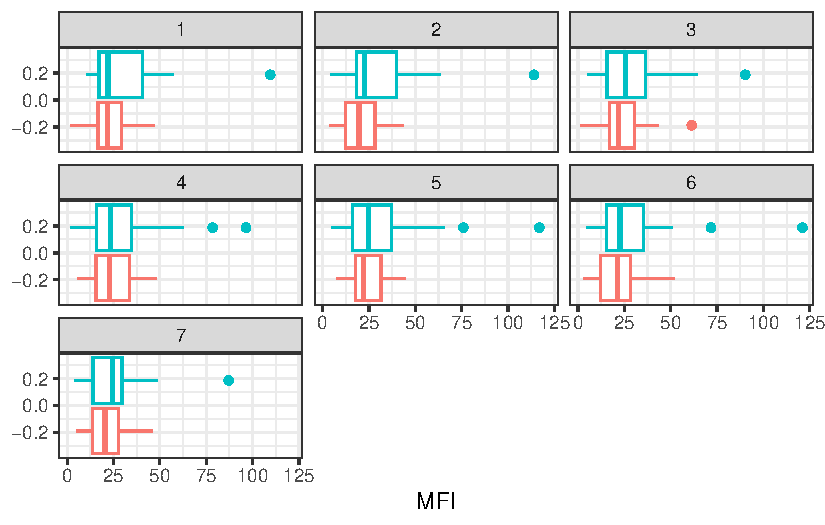
\includegraphics{Class19_files/figure-pdf/unnamed-chunk-26-1.pdf}

}

\end{figure}

\begin{Shaded}
\begin{Highlighting}[]
\FunctionTok{filter}\NormalTok{(ig1, antigen}\SpecialCharTok{==}\StringTok{"FIM2/3"}\NormalTok{) }\SpecialCharTok{\%\textgreater{}\%}
  \FunctionTok{ggplot}\NormalTok{() }\SpecialCharTok{+}
  \FunctionTok{aes}\NormalTok{(MFI, }\AttributeTok{col=}\NormalTok{infancy\_vac) }\SpecialCharTok{+}
  \FunctionTok{geom\_boxplot}\NormalTok{(}\AttributeTok{show.legend =}\NormalTok{ F) }\SpecialCharTok{+}
  \FunctionTok{facet\_wrap}\NormalTok{(}\FunctionTok{vars}\NormalTok{(visit)) }\SpecialCharTok{+}
  \FunctionTok{theme\_bw}\NormalTok{()}
\end{Highlighting}
\end{Shaded}

\begin{figure}[H]

{\centering 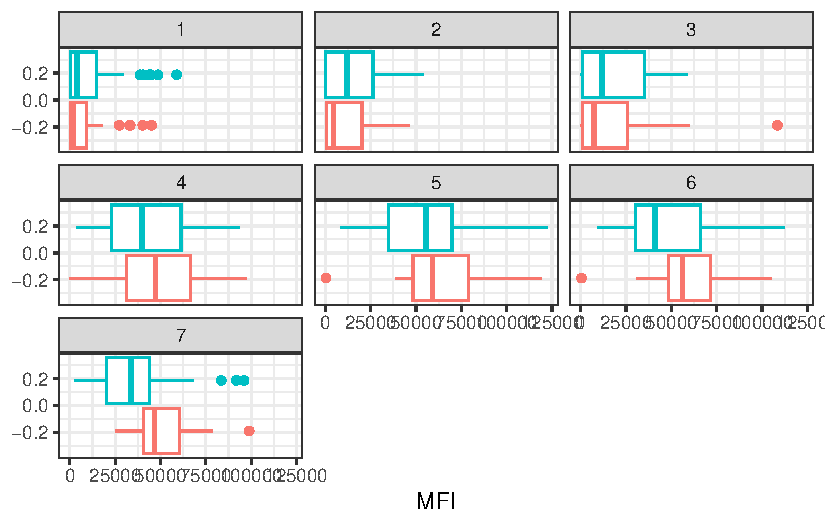
\includegraphics{Class19_files/figure-pdf/unnamed-chunk-27-1.pdf}

}

\end{figure}



\end{document}
